\documentclass{article}%
\usepackage[T1]{fontenc}%
\usepackage[utf8]{inputenc}%
\usepackage{lmodern}%
\usepackage{textcomp}%
\usepackage{lastpage}%
\usepackage[head=40pt,margin=0.5in,bottom=0.6in]{geometry}%
\usepackage{graphicx}%
%
\title{\textbf{Empleados de Bolipuertos exigieron ajuste salarial y amenazaron con cierre}}%
\author{El Nacional Web}%
\date{22/11/2018}%
%
\begin{document}%
\normalsize%
\maketitle%
\textbf{URL: }%
http://www.el{-}nacional.com/noticias/protestas/empleados{-}bolipuertos{-}exigieron{-}ajuste{-}salarial{-}amenazaron{-}con{-}cierre\_260758\newline%
%
\textbf{Periodico: }%
EN, %
ID: %
260758, %
Seccion: %
Protestas\newline%
%
\textbf{Palabras Claves: }%
Caracas, Protestas, Gobierno\newline%
%
\textbf{Derecho: }%
2.3%
, Otros Derechos: %
NO\_TIENE%
, Sub Derechos: %
2.3.4%
\newline%
%
\textbf{EP: }%
SI\newline%
\newline%
%
\textbf{\textit{Los trabajadores se concentraron frente a la sede de Bolivariana de Puertos en Las Mercedes y pidieron la salida del presidente de la institución}}%
\newline%
\newline%
%
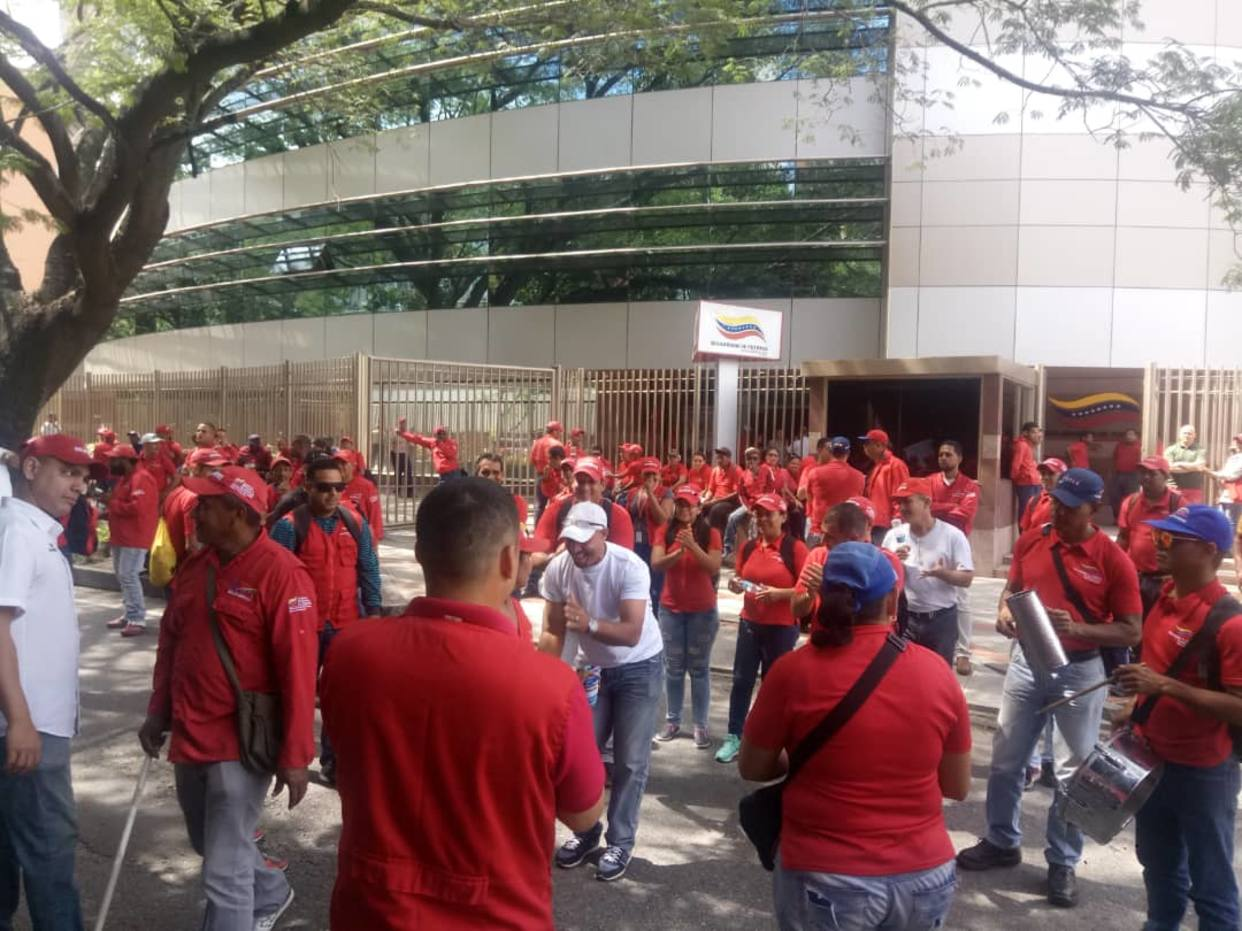
\includegraphics[width=300px]{138.jpg}%
\newline%
%
Los trabajadores de Bolivariana de Puertos (Bolipuertos) realizaron una protesta este jueves en las oficinas ubicadas~en Las Mercedes, Caracas, para exigir reajustes en sus salarios y la salida de Reinaldo Castañeda,~presidente de la institución.%
\newline%
%
"Estamos aquí para reivindicar todos nuestros derechos y beneficios laborales adquiridos por un bloque como la comida y nuestro seguro en las clínicas no nos aceptan ni a nosotros ni a nuestros familiares", dijo un trabajador para~Efecto Cocuyo.%
\newline%
%
"Mi sueldo es de 2.300 bolívares. No hago nada con eso. Tengo dos hijos y mis utilidades fueron de 600 bolívares. Queremos que se respete el sindicato legal. Estoy cansada de este engaño que tiene esta gerencia", dijo una de las manifestantes para el medio digital.%
\newline%
%
Los empleados se congregaron en esta sede y amenazaron con realizar cierres y paralizaciones en varios puertos como La Guaira, La Ceiba y Puerto Cabello si no se les da respuesta con respecto a sus denuncias.%
\newline%
%
"Pedimos la destitución de Castañeda. Somos 6.500 trabajadores que no estamos en contra de nadie~pero nos cansamos. Nos es posible que todas estas personas están pasando trabajos mientras 15 personas en esas oficinas se llenan los bolsillos", aseveró.%
\newline%
%
La institución no se ha pronunciado al respecto de esta protestas y los trabajadores~fueron advertidos con la llegada del Servicio Bolivariano de Inteligencia Nacional (Sebin) si no se iban del lugar.~Un funcionario de Bolipueros recibió las quejas de los trabajadores pero los mismos continuaron frente al edificio.%
\newline%
%
\end{document}